\section{The one-reference problem}\label{app:one}
Fix integers $b\ge1$ and $g\ge1$, a finite integer domain $D=\{0,\ldots,2^b-1\}$ and nonempty groups of magnitudes in $D$. The domain is discrete throughout. Write $B=b+1$. All proofs concern encoded bit patterns. A NaN is a legal word.

Let a magnitude occupy $b$ bits. For binary32, $b=31$ and $a_i=u_i\bmod 2^{31}$, where $u_i$ is the stored unsigned word. The sign bit travels separately. Exponents and fraction fields remain part of $a_i$, including for signed zeros, infinities and NaN payloads. For a stored reference $p\in D=\{0,\ldots,2^b-1\}$ define
\[
 \zz(d)=\begin{cases}2d&d\ge0,\\-2d-1&d<0,\end{cases}
 \qquad w_j(p)=\bitlen\!\left(\max_{i\in G_j}\zz(a_i-p)\right).
\]
Here $\bitlen(0)=0$ and $\bitlen(x)=1+\lfloor\log_2 x\rfloor$ otherwise. Each of the $g$ groups $G_j$ is nonempty. Its minimum and maximum are $l_j,h_j$. The largest possible width is $B=b+1$.

\begin{theorem}[Exact reference selection]\label{th:sweep}
Let $f_j(w)$ be any nondecreasing group cost on $\{0,\dots,B\}$, including byte rounding. For $1\le t<B$ let
\[
 I_{jt}=D\cap[h_j-2^{t-1}+1,\ l_j+2^{t-1}].
\]
At $t=0$ use the singleton $\{l_j\}$ when $l_j=h_j$, and the empty set otherwise. Give $I_{jt}$ weight $f_j(t+1)-f_j(t)$. If $M$ is the maximum total weight of intervals containing one point of $D$, then
\[
 \min_{p\in D}\sum_{j=1}^{g} f_j(w_j(p))=\sum_{j=1}^{g} f_j(B)-M.
\]
A sweep of the interval endpoints returns an attaining reference in $O(gB\log(gB))$ time and $O(gB)$ space after reading the group extrema.
\end{theorem}

The asymmetric $+1$ at the left endpoint matters. For a one-bit group the two encodable differences are $-1$ and $0$. The condition $w_j(p)\le t$ is exactly $p\in I_{jt}$. Summing the weights of the satisfied thresholds telescopes from $f_j(B)$ down to the actual cost. Sorting starts and one-past-ends turns this identity into an algorithm. The supplement proves the endpoint convention, the certificate and the extension to a shared codebook of $k$ references.


The tested layout groups a row of 128 words into sixteen groups of eight. Denote by $s$ the number of nonempty 32-word sign-exception masks, relative to the first word's sign. The residual row length in bytes is
\[
 R(p)=17+4s+\sum_{j=1}^{16} w_j(p).
\]
One descriptor, four reference bytes and twelve width bytes account for the constant 17. The masks are lossless. The shortest alternative $A$ ranges over raw storage, rowwise exponent offsets, four local exponent ranges, and an all-positive-zero escape when admissible. The encoder selects $F(p)=\min\{A,R(p)\}$. A four-byte length and one nonempty-head tag frame all 128 rows. No empirical size table assumes free headers.

\begin{proposition}[Attainable savings and a format lower bound]\label{th:lower}
Write $R_*=\min_p R(p)$, and let $R_0$ be the residual length of any fixed policy. The improvement in the complete row is exactly
\[
 \min(A,R_0)-\min(A,R_*)=[\min(R_0-R_*,A-R_*)]_+ .
\]
Even if every group receives its own free reference, the shortest row with the existing residual header and alternative modes has length
\[
 L_{\rm free}=\min\left\{A,\;17+4s+\sum_j\bitlen(h_j-l_j)\right\}.
\]
It is a lower bound for every shared-reference or multiple-reference scheme using this layout and nonnegative additional overhead. If the residual term inside the braces is at least $A$, the encoder can skip the sweep and emit the winning alternative.
\end{proposition}


\subsection{Thresholds, costs and certificates}
\begin{lemma}[Feasible references for one threshold]\label{lem:threshold}
For $t\ge1$, the group permits width at most $t$ exactly on
$D\cap [h_j-2^{t-1}+1,\ l_j+2^{t-1}]$. Width zero is possible precisely when the group is constant and $p$ is that constant.
\end{lemma}
\begin{proof}
The image of $\zz$ on the consecutive integers from $-2^{t-1}$ through $2^{t-1}-1$ is exactly $\{0,\ldots,2^t-1\}$. Hence all residuals fit if and only if $a_i-2^{t-1}+1\le p\le a_i+2^{t-1}$ for every $i$. Intersect these bounds and $D$. For $t=0$, the only valid residual is zero. This argument includes $p=0$ and $p=2^b-1$.
\end{proof}
\begin{proof}[Proof of the exact reference-selection theorem]
Let $v_{jt}=f_j(t+1)-f_j(t)\ge0$. Since the threshold intervals are nested, a point $p$ belongs precisely to those with $w_j(p)\le t<B$. Thus
\[
 \sum_{t=0}^{B-1}v_{jt}\ind\{p\in I_{jt}\}
 =\sum_{t=w_j(p)}^{B-1}(f_j(t+1)-f_j(t))=f_j(B)-f_j(w_j(p)).
\]
Summing over $j$ proves the threshold identity. For each nonempty integer interval $[L,U]$, add $+v_{jt}$ at $L$ and $-v_{jt}$ at $U+1$. Include $0$ as a candidate of zero initial depth, aggregate coincident events before taking a maximum, and disregard the sentinel $2^b$ as a candidate. The prefix sum is constant up to the next event, so the greatest prefix sum is the maximum feasible depth. Sorting at most $2gB$ events gives the stated time and memory bounds under constant-time endpoint arithmetic. Directly computing frequencies or enumerating all $2^b$ references is unnecessary.
\end{proof}

\paragraph{Verifiable optimum.} A certificate consists of the extrema, a proposed $p$, and the sorted event coordinates with their aggregated signed weights. The verifier independently reconstructs the events, then checks every prefix sum and evaluates the actual width at $p$. Equality of $\sum_jf_j(w_j(p))$ with the constant minus the largest prefix proves optimality. When the sorted multiset is trusted, verification takes $O(gB)$ operations. Independent reconstruction and sorting take $O(gB\log(gB))$. Checking the length at the proposed reference alone would certify only feasibility.

\paragraph{A worked record.} In the five-group example, $g=5$ and $k=5$. At $p=40$ the common value has residual $-16$ with code 31. The outlier has residual $+16$ with code 32. The resulting widths are $(5,5,5,5,6)$. At $p=24$ they are $(0,0,0,0,7)$. Changing $p$ to 25 would give width one to all four constant groups, which already outweighs a one-bit saving in the fifth.


\begin{figure}[ht]
\centering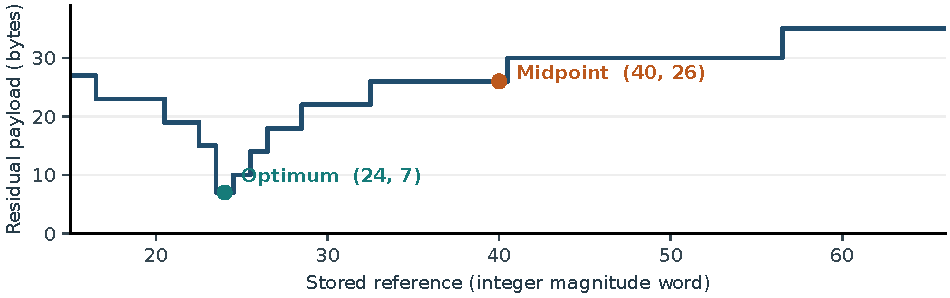
\includegraphics[width=.84\linewidth]{figures/reference_cost.pdf}
\caption{Exact cost of the five-group witness. Each width unit is one byte for a group of eight words.}\label{fig:exampleagain}
\end{figure}

\begin{proposition}[One-outlier separation]\label{th:gap}
For $g\ge2$ groups of eight, $k\ge1$, and $0\le m\le 2^b-1-2^k$, take one magnitude $m+2^k$ and all others $m$, with the outlier in a mixed group. The difference between the midpoint and minimum residual payload is $(g-1)k-1$ bytes.
\end{proposition}
\begin{proof}
At $p=m+2^{k-1}$ the constant groups need width $k$, and the mixed group needs $k+1$. At $p=m$ the common groups cost zero, while the outlier code is $2^{k+1}$ and costs $k+2$. For any other reference, each constant group costs at least one. A width $k$ covers at most $2^k$ consecutive magnitudes, while the mixed group spans $2^k+1$ possible integer positions from its minimum to its maximum inclusive. Hence it costs at least $k+1$ for every reference. Consequently every $p\ne m$ costs at least $(g-1)+(k+1)\ge k+2$. Subtract the two attained values. At $g=2,k=1$ the gap is zero, as the formula predicts.
\end{proof}

\section{Relaxations, screening and more than one reference}\label{app:multiple}
\begin{lemma}[Independent group optimum]\label{lem:span}
For $d=h-l$, $\min_{p\in D}w(p)=\bitlen(d)=\lceil\log_2(d+1)\rceil$.
\end{lemma}
\begin{proof}
For $d=0$ take $p=l$. For $d>0$ a width-$t$ signed code spans at most $2^t-1$ in magnitude difference, so $d\le2^t-1$ is necessary. For the least such $t$, $h-2^{t-1}+1\le l+2^{t-1}$. The left boundary is at most $h$ and the right boundary is at least $l$, so this interval intersects $D$. The threshold lemma supplies a feasible reference. This includes spans $2^t-1$ at equality.
\end{proof}
\begin{proof}[Proof of the complete-format bound]
For numbers $x\ge y$, $\min(A,x)-\min(A,y)$ equals zero for $A\le y$, equals $A-y$ for $y<A<x$, and equals $x-y$ for $A\ge x$. Apply this identity to $x=R_0,y=R_*$. Give each group an independent reference as free side information, keeping the header and sign-mask rules fixed. Group widths can now achieve their separate minima simultaneously, so the formula for $L_{\rm free}$ follows from Lemma~\ref{lem:span}. Choosing an existing alternative is still allowed. If the independent-reference residual length is at least $A$, every genuine residual scheme with this layout is at least as expensive as $A$. The encoder's fixed tie rule gives priority to the alternative, which then determines the same serialized record.
\end{proof}

\paragraph{An even cheaper hypothetical format.} Give the decoder all signs and all group references, including the first reference, for free. Charge only the one-byte descriptor, twelve width bytes and the group payloads. Its per-row floor is
\[
 \min\{A,\ 13+\textstyle\sum_j\bitlen(h_j-l_j)\}.
\]
This is an attainable length with that side information, and a lower bound when it must be transmitted. All nonempty heads retain the original five framing bytes. The aggregate is 142,111,471 bytes, exceeding the bit-shuffled control by just 17,574 bytes (0.0124\% of the control). This second gap is sensitive to framing and checkpoint mix. A different entropy code for the widths, variable group boundaries, or another alternative row mode would define a different family.

\subsection{The optimum with a shared codebook}
Let $P\subseteq D$ be a set of at most $k$ references, $k\ge1$. Each group may select a reference independently. Suppose that headers and reference-index costs are fixed once $k$ is chosen. A fixed selector of $\lceil\log_2 k\rceil$ bits per group satisfies this assumption. Variable costs depending on the selected index require another objective.
\begin{theorem}[Codebook reduction]\label{th:multiple}
For the costs in the one-reference theorem, minimizing
$\sum_j\min_{p\in P} f_j(w_j(p))$ is equivalent to maximizing the total interval weight hit by at least one point of $P$. Some optimum uses only $0$ and left endpoints of nonempty threshold intervals.
\end{theorem}
\begin{proof}
The interval family is nested for each group, and $f_j$ is nondecreasing. The thresholds hit by any point in $P$ are exactly the thresholds at or above $\min_{p\in P}w_j(p)$. Telescope the cost as before. For the second statement, remove any point that hits nothing. For each remaining point replace it with the largest left endpoint of the intervals that it hits. That value is no larger than the point and still lies in every previously hit interval. Coincident replacements can be merged. With zero total weight the point $0$ is sufficient.
\end{proof}

\paragraph{Dynamic program and certificate.} Sort the $m$ distinct candidate coordinates as $x_1<\cdots<x_m$. Use a sentinel $x_0=-1$. For $i<j$ let
\[
 H(i,j)=\sum_{[L,U]}v_{LU}\ind\{x_i<L\le x_j\le U\}.
\]
If the previous rightmost selected point is $x_i$, an interval containing $x_j$ is new precisely when $L>x_i$. Indeed, if $L\le x_i$ it already contains $x_i$, while if $L>x_i$ every earlier point is too far left. With $D_1(j)=H(0,j)$, the recurrence
\[
 D_r(j)=\max_{i<j}\{D_{r-1}(i)+H(i,j)\}
\]
therefore computes the best covered weight with $r$ ordered points ending at $x_j$. Unreachable states are $-\infty$. Take the maximum over $r\le\min(k,m)$ and $j$, allowing the empty solution of value zero. Backpointers give attaining references. For $n$ nonempty threshold intervals one may tabulate $H$ in $O(m(n+m))$ time: for each right candidate bin the active interval weights by their left endpoints and take suffix sums. The dynamic program then costs $O(km^2)$ time, with $O(m^2+km)$ space including reconstruction. Classical partial interval hitting admits other algorithms \cite{hitting}. Our use is an exact benchmark for this byte cost. The multi-reference formula has been checked on finite examples. The corpus measurements executed the single-reference encoder.

\section{Word identity and the limits of geometric evidence}\label{app:words}
\begin{proposition}[Lossless transport through a deterministic update]\label{th:transport}
Let $E,D$ encode and decode a state of machine words with $D(E(x))=x$ on all reachable states. Consider a deterministic native transition and output $(x',y)=T(x,u)$ whose other state, arithmetic environment and input sequence are identical in both runs. The wrapped transition forms $(x',y)=T(D(c),u)$ and stores $E(x')$. Starting from $c_0=E(x_0)$ yields equal native state and output words at every step.
\end{proposition}
\begin{proof}
Initially the decoded state agrees by assumption. At any step equal input and resident auxiliary state give identical arguments to $T$ and hence identical output and next native state. Applying $D\circ E$ preserves that state for the next step. This induction also covers a sampler if its state and random draws agree. Integer residual storage satisfies the premise because $p+\zz^{-1}(\zz(a-p))=a$ and XOR with a saved sign mask is its own inverse. The exponent modes invert integer offsets and copy every other field. Raw storage and the positive-zero escape have explicit inverses. Bytewise equality avoids the ambiguity of floating-point comparisons at signed zero or NaNs.
\end{proof}
Changing reduction order, floating-point contraction, sampler state or the native transition changes the hypotheses. The storage replay in this paper checks the codec premise on the archived words. It does not execute a new online model transition.

\begin{theorem}[A high-energy rank-one component can hide arbitrary bits]\label{th:rank}
For positive integers $m,n$ and $1\le s\le23$, there are $2^{smn}$ distinct positive binary32 matrices $X$ for which the rank-one matrix $J=\mathbf1\mathbf1^\top$ satisfies
\[
 \frac{\lVert X-J\rVert_F^2}{\lVert X\rVert_F^2}
 \le ((2^s-1)2^{-23})^2 .
\]
Every injective binary representation has worst-case length at least $smn$ bits on this family. A prefix-free representation has uniform expected length at least $smn$ bits.
\end{theorem}
\begin{proof}
Independently choose $d_{ij}\in\{0,\ldots,2^s-1\}$ and set $X_{ij}=1+2^{-23}d_{ij}$. Binary32 represents all of these numbers exactly within the same exponent bin. The numerator is at most $mn((2^s-1)2^{-23})^2$ and the denominator is at least $mn$. Fewer than $2^{smn}$ binary strings have length strictly below $smn$, which proves the worst-case bound. For a prefix code of lengths $L_i$, Kraft's inequality and convexity give $2^{-\mathbb E L}\le \mathbb E2^{-L}\le2^{-smn}$ under the uniform law.
\end{proof}
For $s=12$, the relative squared error is below $2.39\times10^{-7}$ while 12 freely chosen bits per entry remain. This construction is a counting obstruction to using an approximation score as a lossless code-length guarantee. Structured states outside the family can compress much further.

\section{Records, protocols and checks}\label{app:experiment}
\subsection{Exactly what is on the wire}
A layer dump stores sixteen little-endian FP32 heads. Within a head, the row decoder reads 128 consecutive self-delimiting records. For a nonzero head, the four-byte unsigned payload length precedes a one-byte head tag and the records. An all-positive-zero head uses a zero length and no head tag or row bytes. The dense baseline costs exactly 65,536 bytes per head. The code checks the machine byte order before replay.

\begin{center}\small
\begin{tabular}{ll}\toprule
Row mode & Serialized bytes per 128-word row \\ \midrule
Raw & $1+512$ \\
One exponent minimum and width $e$ & $386+16e$ \\
Four local minima and widths $e_t$ & $391+4\sum_{t=1}^4e_t$ \\
Integer magnitude residual & $17+4s+\sum_{j=1}^{16}w_j$ \\
All positive zeros & $1$ \\ \bottomrule
\end{tabular}
\end{center}
Exponent offsets take the unsigned bit length of the exponent span. The sign and 23 fraction bits occupy three bytes per word. In the residual mode the reference word holds a 31-bit reference magnitude and the sign of the first word. Each 32-word tile stores a four-byte XOR sign mask only when some sign differs from the reference sign. Six bits per group width suffice for values 0 through 32, even when residuals reach 32 bits. Bit packing is least-significant bit first. The baseline midpoint is the floor of $(\min a+\max a)/2$ evaluated in widened integer arithmetic. The lower median is order statistic 64 among 128 values. On ties the nonzero encoder chooses raw, then row exponents, then local exponents, then residuals. This tie convention also allows the screened encoder to reproduce the unscreened stream byte for byte. Row records are sequentially parseable. A random-row offset table would incur additional bytes.

The whole-head controls use the same granularity and wrapper accounting as each other. A tag identifies the transformation and compressor, and a four-byte unsigned length delimits the frame. The byte shuffle concatenates the four byte lanes of the entire head. The bit shuffle transposes contiguous blocks of 256 words into 32 bit planes. A single Zstandard frame covers the transformed head. Each baseline falls back to the native payload if compression fails to shorten it. Sizes describe these explicitly implemented serializations. No indexes across heads, allocator capacity, Python objects or resident model weights are included.

\subsection{Results by checkpoint and recurrent layer}
\begin{table}[ht]\centering\small
\caption{Saving from replacing the midpoint with the exact reference. Each checkpoint comprises 864 heads and 110,592 rows. Retained is the complete-format gain divided by the residual-only gain.}\label{tab:checkpoints}
\begin{tabular}{rrrrr}\toprule Token & Residual bytes saved & Frame bytes saved & Retained & Rows shortened \\ \midrule
\tabinput figures/checkpoints.tex 
\bottomrule\end{tabular}
\end{table}
\begin{figure}[ht]\centering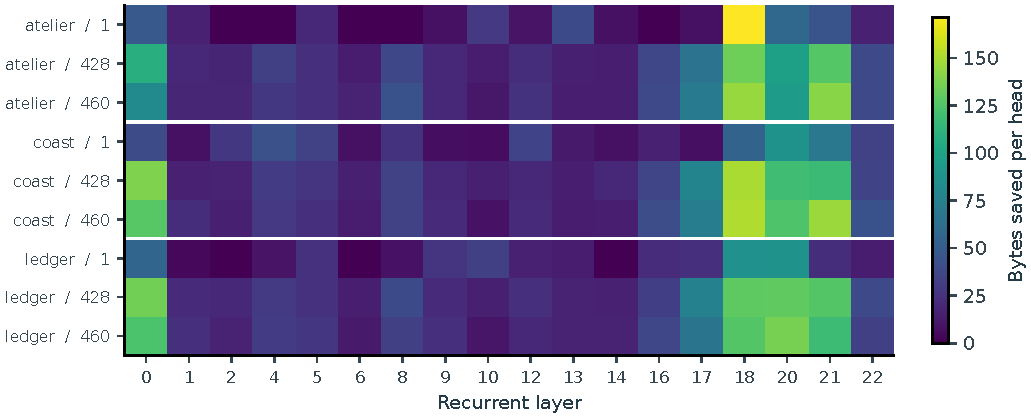
\includegraphics[width=\linewidth]{figures/layers.pdf}
\caption{Complete-format savings from exact reference selection. Each cell is the mean difference in bytes over the 16 heads of the indicated layer, trace and token. All 18 recurrent layers are included. Early checkpoint measurements differ visibly by layer.}\label{fig:layer}
\end{figure}
\begin{table}[ht]\centering\small
\caption{Dependence on the saved token. The last two columns compare head frames. Free sides is the lower bound with all group references and signs supplied for free.}\label{tab:free}
\begin{tabular}{rrrrr}\toprule Token & Fixed-header floor & Free sides & Optimal local & Bit shuffle + Zstd \\ \midrule
\tabinput figures/floors.tex 
\bottomrule\end{tabular}
\end{table}
The residual mode wins 3,858 rows at the midpoint and 39,694 under optimal selection. A rise in the number of wins can accompany a small change in bytes because a new residual winner must first cross the competing exponent record. Table~\ref{tab:checkpoints} quantifies this effect. The 17,574-byte gap in the more permissive relaxation is an aggregate across the three equally weighted positions. Table~\ref{tab:free} shows why this number cannot be extrapolated to a steady-state distribution of token ages.

\begin{figure}[ht]\centering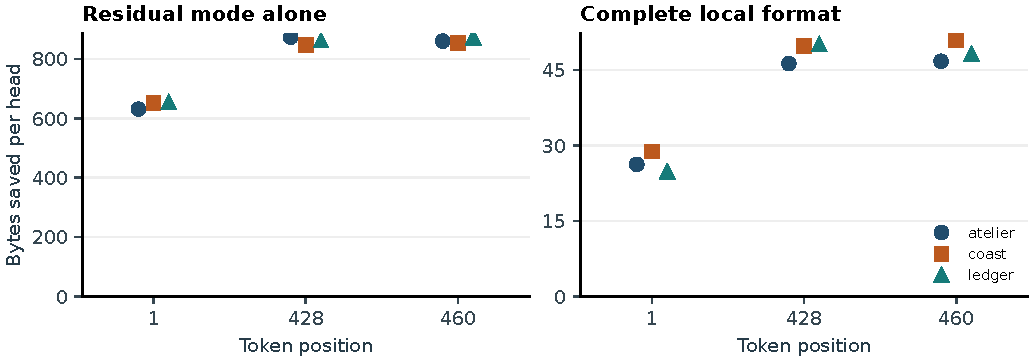
\includegraphics[width=.94\linewidth]{figures/mode_competition.pdf}
\caption{Savings from the optimal reference before and after mode selection. Each point averages 288 heads at one trace and checkpoint. Each panel has its own byte scale.}
\end{figure}
\begin{table}[ht]\centering\small
\caption{All measured lossless controls. Sizes include head framing for each coded representation.}
\begin{tabular}{lrrr}\toprule Method & Bytes & Bits per word & Saved (\%)\\\midrule
\tabinput figures/sizes.tex
\bottomrule\end{tabular}
\end{table}
\subsection{An adaptive head frame}\label{app:mixed}
For head $i$, let $a_i$ and $b_i$ be the complete serialized local-optimal and bit-shuffle/Zstandard lengths. We concatenate one unsigned selector byte followed by the chosen intact frame. Selector zero indicates the local format; selector one indicates bit shuffle, including its own raw fallback. Both inner formats already delimit their payload with a four-byte little-endian length, so a decoder can walk the concatenation with no external offsets. Ties select bit shuffle. For $H$ heads the allocation is exactly $H+\sum_i\min(a_i,b_i)$. Against always storing the bit-shuffled frame, the net gain is $\sum_i[b_i-a_i]_+-H$. With this wrapper, local optimality of choosing the shorter frame follows from separability over heads.

\begin{table}[ht]\centering\small
\caption{Fresh serialization and bytewise readback of the two-format stream. Each token position contributes 864 heads. All byte totals include the one-byte outer selector per head.}
\begin{tabular}{rrrr}\toprule Token position & Local selected & Shuffle selected & Mixed bytes\\\midrule
1 & 0 & 864 & 42,040,298\\
428 & 777 & 87 & 49,384,814\\
460 & 745 & 119 & 49,310,794\\\midrule
All & 1,522 & 1,070 & 140,735,906\\\bottomrule\end{tabular}
\end{table}
We ran the original four-policy replay and the mixed encoder on all 42,467,328 native FP32 words. For each head the census replay matched the stored counts and the mixed decoder matched the raw input and the recorded SHA-256. The mixed encoder constructs both candidates in memory. The extra encoding latency, peak transient memory and online access pattern are open performance questions.

\subsection{CPU microbenchmark and historical inference context}
\begin{table}[ht]\centering\small
\caption{In-memory encode-only timings for the bundled 162-head subset (10,616,832 input bytes per pass). Range is the minimum and maximum across eight post-warm-up passes. MB/s uses decimal input megabytes and median pass time.}\label{tab:time}
\begin{tabular}{lrrr}\toprule Reference policy & Median (ms) & Range (ms) & MB/s \\ \midrule
\tabinput figures/timings.tex 
\bottomrule\end{tabular}
\end{table}
One head per (trace, token, layer) was retained in the portable subset. Use zero-based layer ordinal $j$ in the sorted recurrent-layer list and trace ordinal $i$ in (atelier, coast, ledger). The retained head index is $(j+5i)\bmod16$. Selection is independent of the values and identical across token positions for each trace and layer. Every method encoded the same 162 heads. The timed C++ process was pinned to one logical CPU on an AMD EPYC 9V74 and built with GCC 14.2, \texttt{-O3 -std=c++17}. One unrecorded warm-up pass per policy preceded eight timed passes per policy. Starting order rotated across repeats. Input was already resident. The timed loop encoded into a preallocated buffer, including framing. A checksum consumed all output bytes outside the timer. Typical full verification also requires space for the 162 MiB original corpus, compiler output and per-row CSVs. No GPU or inference engine is needed to reproduce the codec results.

A separate historical integration \cite{archive} measured the \emph{midpoint} local format in Qwen3.5-0.8B-Q4\_K\_M, using four pinned CPU cores. Peak recurrent-matrix allocation was 18,874,368 bytes natively and 16,760,064 bytes in a locally fused implementation. Process peak RSS was 837,459,968 and 832,233,472 bytes respectively. A separate three-repeat timing protocol reported medians of 13.732 and 20.386 seconds. This historical result supports the decision to measure bytes and runtime separately. The current Q4\_0 snapshot study uses a different quantization and traces, and its new optimizer was run offline.

\subsection{Reproduction and numerical checks}
The companion notebook includes the complete per-head census, raw words for the 162-head portable replay, the C++ codec, an independent integer verifier and all plot sources. Its default CPU run regenerates the tables and figures from per-head observations and verifies the portable subset against those observations. The optional full-data input contains the original words for all 2,592 heads. Supplying it to the notebook repeats the entire census. The archived capture names are \texttt{Qwen\_GDN\_Full\_State\_Lossless\_Evidence.zip} and \texttt{Qwen\_GDN\_Full\_State\_Lossless\_Results.zip}. Sorted census order is trace, token, layer and head. For exact baseline sizes the reference environment used python-zstandard 0.25.0 with libzstd 1.5.7. The companion records zlib and other runtime versions. The portable replay compares the pinned local codec independently of external compressor versions.

\begin{itemize}\setlength\itemsep{1pt}
\item The Python verifier enumerates all 4,096 ordered four-symbol records over an eight-symbol alphabet with two groups, checking both one and two references by exhaustive codebook search. It also checks 180 fixed-seed four-group records each with one, two and three references, 116 outlier identities, and extreme 31-bit endpoints.
\item An independent C++ loop enumerates the same 4,096 records expanded to sixteen groups and compares the production endpoint sweep against direct reference enumeration. Across 128 constructed rows, 512 round trips exercise all five row modes and include both signs of zero, denormals, infinities and NaN payloads.
\item The census runner verifies every selected row length, per-row dominance, the complete-format identity and the independent-span floor. It decodes every serialized head and checks it against the raw bytes. The four general-purpose controls have separate inverse transformations.
\end{itemize}

The corpus consists of model-state words. It includes no model weights or user conversation transcripts. The Qwen base model card identifies its Apache 2.0 license \cite{qwen}. Shorter exact checkpoints can lower storage requirements, while the ability to reconstruct all state bits means that ordinary access restrictions for the uncompressed state also apply to its encoded form. A language model assisted with the derivations, manuscript and implementation. The proofs specify the claims supported by finite computation and distinguish the historical engine evidence from the new results.
